\documentclass{standalone}
\usepackage{tikz}
\definecolor{c0}{HTML}{b0702b}
\definecolor{c1}{HTML}{b56769}
\definecolor{c2}{HTML}{B2746B}
\definecolor{c3}{HTML}{86a86c}
\definecolor{c4}{HTML}{697fa0}
\definecolor{c5}{HTML}{896190}
\definecolor{c6}{HTML}{37537C}
\def\xzero{-0.55}
\def\xone{3.7}
\def\xonehalf{4.25}
\def\xtwo{6.4}
\def\y{+0.42}
\def\xthree{7.4}
\def\xfour{9}
\def\xfive{4.4}
\def\xsix{13}
\def\xseven{8.3}
\begin{document}

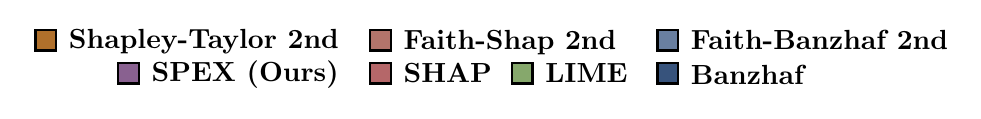
\begin{tikzpicture}
\useasboundingbox (-.05,0.05) rectangle (11.7,.85);
    \draw[fill=c5, thick] (.6+0.5,0.4) rectangle (0.86+0.5,0.14);
    \node[anchor=west] at (0.9+.5,0.26) {\textbf{SPEX (Ours)}};

    \draw[fill=c3, thick] (.6+\xone+1.8,0.4) rectangle (0.86+\xone+1.8,0.14);
    \node[anchor=west] at (0.9+\xone+1.8,0.28) {\textbf{LIME}};

    \draw[fill=c1, thick] (.6+\xonehalf+\xzero,0.4) rectangle (0.86+\xonehalf+\xzero,0.14);
    \node[anchor=west] at (0.9+\xonehalf+\xzero,0.28) {\textbf{SHAP}};


    \draw[fill=c2, thick] (.6+\xonehalf+\xzero,0.4+\y) rectangle (0.86+\xonehalf+\xzero,0.14+\y);
    \node[anchor=west] at (0.9+\xonehalf+\xzero,0.24+\y) {\textbf{Faith-Shap 2nd}};

    \draw[fill=c0, thick] (.6+\xzero,0.4+\y) rectangle (0.86+\xzero,0.14+\y);
    \node[anchor=west] at (0.9+\xzero,0.25+\y) {\textbf{Shapley-Taylor 2nd}};

    \draw[fill=c4, thick] (.2+\xseven+\xzero,0.4+\y) rectangle (0.46+\xseven+\xzero,0.14+\y);
    \node[anchor=west] at (0.5+\xseven+\xzero,0.28+\y) {\textbf{Faith-Banzhaf 2nd}};
    
    \draw[fill=c6, thick] (.2+\xfour-1.25,0.4) rectangle (0.46+\xfour-1.25,0.14);
    \node[anchor=west] at (0.5+\xfour-1.25,0.25) {\textbf{Banzhaf}};

\end{tikzpicture}

\end{document}